\chapter{Validation}\label{ch:valid}

\epigraph{The logic of validation allows us to move between the two limits of dogmatism and skepticism.}{\textit{The Model of the Text: Meaningful Action Considered as a Text\\
Paul Ric\oe{}ur}}

\minitoc

\lettrine{\color{theme}{N}}umerical simulations are collected in this chapter to assess the correctness of the proposed formulation for flexible multibody dynamics in pH form. Two main sections compose the chapter: the first one is dedicated to systems composed of beams, the second involves  thin plates as mechanical components. The {\sc{Firedrake}} python library \cite{rathgeber2017firedrake} is employed to construct the finite-dimensional discretization.

\section{Beam systems}
The examples presented in this section make use of Euler Bernoulli beam model \eqref{eq:EB_sys}. To discretize the system, Lagrange polynomial of order one and Hermite polynomials of order 3 are used for $v_f^x$ and $v_f^y$ respectively. Discontinuous Galerkin elements of order 0 and 1 are selected for $n_x$ and $m_{x}$ respectively. This choice corresponds to the HerDG1 element \eqref{eq:HerDG1} for the bending behavior and to the CGDG element \eqref{eq:CGDG} for the truss behavior.  \\
 
The first example concerns the computation of eigenvalues of a four bar mechanism for different geometrical configuration. The second example is a rotating crank-slider. In this case the non-linearities cannot be neglected. The third example is a hinged beam undergoing external excitations so that the out-of-plane motion becomes important.   


\subsection{Linear analysis of a four-bar mechanism}

\begin{figure}[tb]
	\centering
	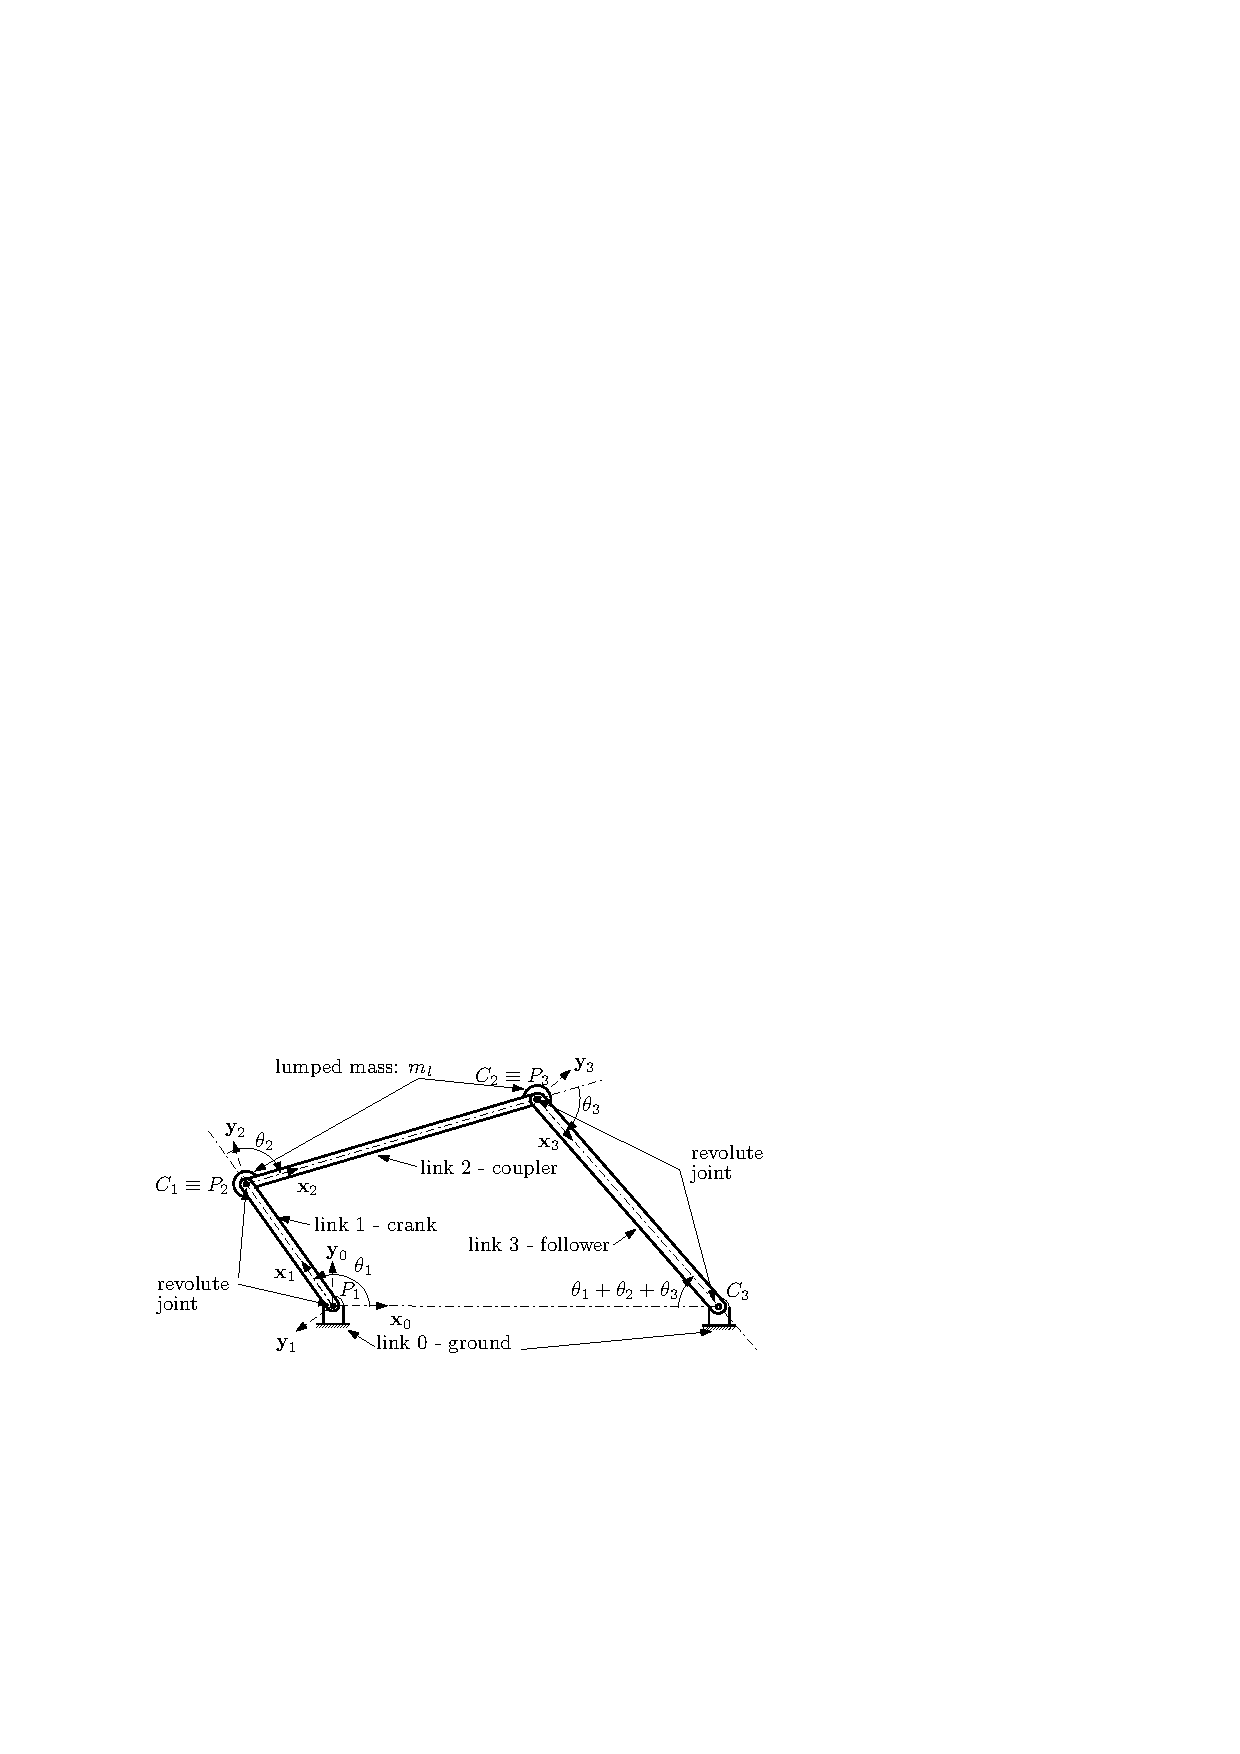
\includegraphics[width=0.6\textwidth]{part_4/validation/EB/fourbars.pdf} 
	\hspace{.3cm}
	\includegraphics[width=0.35\textwidth]{part_4/validation/EB/block_4bars.eps} 
	\caption{Four bar mechanism illustration (left) and block diagram used for the eigenvalues analysis (right)}
	\label{fig:4bars}
\end{figure}

\begin{table}[bt]
	\centering
	% table caption is above the table
	\caption{Four-bar mechanism links properties: each link is a uniform beam with mass density $\rho=2714\,[\mathrm{kg}/\mathrm{m}^3]$ and Young modulus $E=7.1\,10^{10}\,[\mathrm{N}/\mathrm{m}^2]$. }
	\label{tab:data_4bars}       % Give a unique label
	% For LaTeX tables use
	\begin{tabular}{lllll}
		\hline\noalign{\smallskip}
		$i$ & $0$ &  $1$ &  $2$ &  $3$  \\
		\noalign{\smallskip}\hline\noalign{\smallskip}
		Name & ground & crank & coupler & follower \\ 
		Length $L_i\,[\mathrm{m}]$ & $0.254$ & $0.108$ & $0.2794$ & $0.2705$\\
		Cross section $A_i\,[\mathrm{m}^2]$ & $-$ & $1.0774\,10^{-4}$ & $4.0645\,10^{-5}$ & $4.0645\,10^{-5}$ \\
		Flexural rigidity $(EI)_i\,[\mathrm{Nm}^2]$ & $-$ & $11.472$ & $0.616$ & $0.616$ \\
		\hline
	\end{tabular}
\end{table}

The four-bar mechanism has one degree of freedom and represents a closed chain of bodies. The data are taken from \cite{kitis1990natural,chebbi2017} are recalled in Table \ref{tab:data_4bars}. In Fig. \ref{fig:4bars} the mechanism and the corresponding block diagram used for constructing the final pH system with transformer interconnections between subsystems are presented. The lumped masses are directly included in the coupler and follower model considering a simple modification of the rigid mass matrix
\begin{equation*}
\mathbf{M}_{rr}^{i + m_l}[1:2,1:2] = \mathbf{M}_{rr}^{i}[1:2,1:2] + \mathbf{I}_{2\times 2} m_l,
\end{equation*} 
where $i=2,3$ denotes the coupler or follower model. Given a certain crank angle $\theta_1$ the relative angles between the different links are found by solving the two kinematic constraints
\begin{align*}
L_1 \cos(\theta_1)+ L_2 \cos(\theta_1+\theta_2)+ L_3 \cos(\theta_1+\theta_2+\theta_3) &=L_0, \\
L_1 \sin(\theta_1)+L_2 \sin(\theta_1+\theta_2)+L_3 \sin(\theta_1+\theta_2+\theta_3) &=0.
\end{align*} 
Once the angles describing the geometrical configuration are known, the transformer interconnection \eqref{eq:int_hinge} is applied to insert a revolute joint between adjacent links. For the deformation field a cantilever condition is imposed for each beam. The resulting system is then constrained to ground by imposing to following equalities
\begin{equation*}
\mathbf{v}_{P_1} = \mathbf{0}, \quad \omega^z_{P_1} = 0, \quad \mathbf{v}_{C_3} = \mathbf{0}.
\end{equation*}
The resulting system is expressed in pH form as $\mathbf{E}\dot{\mathbf{e}} = \mathbf{J} \mathbf{e}$. The eigenfrequencies are then found by solving the generalized eigenvalue problem $\mathbf{E}\bm{\Phi} = \mathbf{J} \bm{\Phi \Lambda}$. Since $\mathbf{J}$ is skew-symmetric the eigenvalues will be imaginary $\bm{\Lambda} = j \bm{\Omega}$. The first three pulsations  are reported in Fig. \ref{fig:omega_4bars} for different values of the crank angle $\theta_1$. The results match those of \cite{chebbi2017} (labeled as TITOP in the figure), assessing the validity of the linear model.

\begin{figure}[tb]
	\centering
	\includegraphics[width=0.49\textwidth]{part_4/validation/EB/FourBar_Om12_Chebbi.eps} 
	\includegraphics[width=0.49\textwidth]{part_4/validation/EB/FourBar_Om3_Chebbi.eps} 
	\caption{Eigenvalues $\omega_i, \ i=1,2,3$ for the four bar mechanism for varying crank angle.}
	\label{fig:omega_4bars}
\end{figure}

\subsection{Rotating crank-slider}
To verify the non-linear planar model a crank-slider rotating at high speed is considered. The example is retrieved form \cite{ellenbroek2018}.  The crank is considered as rigid, with length $L_{\text{cr}} = 0.15 \ [\mathrm{m}]$ and rotates at a constant angular rate $\omega_{\text{cr}} = 150 \ [\mathrm{rad/s}]$. The flexible coupler has length $L_{\text{cl}} = 0.3 \ [\mathrm{m}]$ and a circular cross section whose diameter is $d_{\text{cl}} = 6 \ [\mathrm{mm}]$. Its Young modulus and density are given by $E_{\text{cl}}=0.2 \ 10^{12} \ [\mathrm{Pa}]$, and $\rho_{\text{cl}}=7870 \ [\mathrm{kg/m}^3]$. The slider has a total mass equal to half the mass of the coupler $m_{\text{sl}} = 0.033 \ [\mathrm{kg}]$. A simply supported condition is supposed for the coupler deformation field. This choice is motivated by the fact that the slider has a large inertia and does not allow elastic displacement at the tip.

\begin{figure}[tb]
	\centering
	\includegraphics[width=0.5\textwidth]{part_4/validation/EB/cr_slider.eps} 
	\includegraphics[width=0.4\textwidth]{part_4/validation/EB/block_crslider.eps} 
	\caption{Crank slider illustration (left) and block diagram (right)}
	\label{fig:crsl}
\end{figure}

An illustration of the system and the block diagram used to construct the model are provided in Fig. \ref{fig:crsl}. To construct the crank slider a transfomer interconnection is first used to connect the slider to the flexible coupler. The motion of the slider is then computed in the coupler reference frame. Then the sliding constraint, that requires the vertical velocity of the slider to be null in the inertial frame, is imposed as follows
\[
0 = \sin(\theta_{P_1}) v^x_{P_2} + \cos(\theta_{P_1}) v^y_{P_2} = \mathbf{R}_y(\theta_{P_1}) \mathbf{v}_{P_2},
\]
where $\mathbf{R}_y$ is the second line of the rotation matrix and ${\theta}_{P_1}$ is the angle defining the orientation of the coupler. The rigid crank velocity at the endpoint  
\begin{equation*}
\mathbf{v}_{\text{cr}}(t) = -\omega_{\text{cr}} L _{\text{cr}} \sin(\omega_{\text{cr}} t) \widehat{\mathbf{X}} + \omega_{\text{cr}} L _{\text{cr}} \cos(\omega_{\text{cr}} t) \widehat{\mathbf{Y}}
\end{equation*} 
has to be written in the coupler reference frame to get the input
\begin{equation*}
\mathbf{u}_{\text{cl}} = \mathbf{R}(\theta_{P_1})^\top \mathbf{v}_{\text{cr}}.
\end{equation*}
The resulting system is a quasi linear index-2 DAE of the form
\begin{equation*}
\begin{bmatrix}
\mathbf{M} & \mathbf{0} & \mathbf{0} \\
\mathbf{0} & \mathbf{0} & \mathbf{0} \\
\mathbf{0} & \mathbf{0} & \mathbf{0} \\
\end{bmatrix}
\begin{bmatrix}
\dot{\mathbf{e}} \\ \dot{\bm{\lambda}}_0 \\ \dot{\bm{\lambda}}_u \\
\end{bmatrix}= 
\begin{bmatrix}
\mathbf{J}(\mathbf{e}) & \mathbf{G}_0^\top(\theta_{P_1}) & \mathbf{G}_u^\top \\
-\mathbf{G}_0(\theta_{P_1}) & \mathbf{0} & \mathbf{0} \\
-\mathbf{G}_u & \mathbf{0} & \mathbf{0} \\
\end{bmatrix}
\begin{bmatrix}
\mathbf{e} \\ \bm{\lambda}_0 \\ \bm{\lambda}_u \\
\end{bmatrix} + 
\begin{bmatrix}
\mathbf{0} \\ \mathbf{0} \\ \mathbf{R}(\theta_{P_1})^\top \\
\end{bmatrix}
\mathbf{v}_{\text{cr}}.
\end{equation*}


\begin{figure}[tb]
	\centering
	\includegraphics[width=0.45\textwidth]{part_4/validation/EB/uM_disp.eps} 
	\includegraphics[width=0.45\textwidth]{part_4/validation/EB/wM_disp.eps} 
	\caption{Coupler midpoint horizontal (left) and vertical (right) displacement}
	\label{fig:defM_crsl}
\end{figure}

Setting the initial conditions properly is of utmost  importance for a DAE solver. For this problem the beam is supposed undeformed at the initial time. The initial conditions for the rigid movement are then found using basic kinematics considerations.  The system is then solved using the IDA algorithm available in the Assimulo library \cite{assimulo2015}. The computational performance for this test case are reported in Tab. \ref{tab:comp_perf_crslider} In Fig. \ref{fig:defM_crsl} the midpoint deformation displacement $u_f^x(L_{\text{cl}/2}),\; u_f^y(L_{\text{cl}/2})$, normalized with respect to the coupler length, is reported. The resulting vertical displacement is in accordance with the results presented in \cite{ellenbroek2018}. The horizontal displacement exhibits high oscillations because of the higher eigenfrequencies of the longitudinal movement. This is due to the fact that null initial conditions are imposed on the deformation \cite{simeon2006}. In order to obtain a smoother solution, the initial deformation has to be computed from the rigid initial condition.


\begin{table}[tb]
	\centering
	% table caption is above the table
	\caption{{Computational performances for the crank slider.}}
	\label{tab:comp_perf_crslider}       % Give a unique label
	% For LaTeX tables use
	\begin{tabular}{cccc}
		\hline\noalign{\smallskip}
		Solver & Elapsed simulation time & Average $\Delta t$ & Final time \\
		\noalign{\smallskip}\hline\noalign{\smallskip}
		IDA & $12.14\; \mathrm{[s]}$ & $4.98 \, 10^{-7} \; \mathrm{[s]}$ & $0.053 \, 10^{-4} \; \mathrm{[s]}$\\
		\hline
	\end{tabular}
\end{table}

\subsection{Hinged spatial beam}
A spatial beam rotating about a spherical joint is considered (see Fig. \ref{fig:beam_3D}). This example was considered in \cite{cardona2000,ellenbroek2018}. The physical parameters are briefly recalled in Table \ref{tab:data_3Dbeam}. The spherical joint constraint is imposed by setting to zero the linear velocity, while a cantilever is imposed for the deformation field as the tip is free. For the first $10.2 \; [\mathrm{s}]$ a torque $ M_z =200 \; [\mathrm{N/mm}]$ is applied about the vertical axis. Then, an impulsive force $ F_z =100 \; [\mathrm{N}]$ is applied at the tip of the beam at $15 \; [\mathrm{s}]$, to excite the out-of-plane movement. The system is solved using an implicit Runge-Kutta method of the Radau IIA family {(see Tab. \ref{tab:comp_perf_hinged} for the computational performance of this test case)}. The simulation results, provided in Fig. \ref{fig:H_omega}, correspond to the total energy and the angular velocity measured in the inertial vertical direction. The result matches with the provided references. Indeed the non-linearities associated to the gyroscopic terms are small as the maximum angular velocity is equal to $0.1 \; [\mathrm{rad/s}] \approx 5 \; [\mathrm{deg/s}]$. 

\begin{figure}[tb]
	\centering
	\includegraphics[width=0.45\textwidth]{part_4/validation/EB/rotbeam_3D.eps} 
	\caption{Spatial beam on a spherical joint.}
	\label{fig:beam_3D}
\end{figure}

\begin{figure}[tb]
	\centering
	\includegraphics[width=0.45\textwidth]{part_4/validation/EB/H_3Dbeam.eps} 
	\includegraphics[width=0.45\textwidth]{part_4/validation/EB/omega_zI.eps} 
	\caption{Simulation results: kinetic energy (left) and angular velocity about the vertical inertial direction (right).}
	\label{fig:H_omega}
\end{figure}

\begin{table}[tb]
	\centering
	% table caption is above the table
	\caption{Physical parameters for the hinged spatial beam.}
	\label{tab:data_3Dbeam}       % Give a unique label
	% For LaTeX tables use
	\begin{tabular}{lllll}
		\hline\noalign{\smallskip}
		Length & Cross section & Inertia moment & Density & Young modulus \\
		\noalign{\smallskip}\hline\noalign{\smallskip}
		141.45 $[\mathrm{mm}]$ & 9.0 $[\mathrm{mm}^2]$ & 6.75 $[\mathrm{mm}^4]$ & 7800 $[\mathrm{kg/mm}^3]$ & 2.1 $10^6 \ [\mathrm{N/m}^2]$  \\
		\hline
	\end{tabular}
\end{table}


\begin{table}[tb]
	\centering
	% table caption is above the table
	\caption{Computational performances for the hinged spatial beam.}
	\label{tab:comp_perf_hinged}       % Give a unique label
	% For LaTeX tables use
	\begin{tabular}{cccc}
		\hline\noalign{\smallskip}
		Solver & Elapsed simulation time & Average $\Delta t$ &  Final time \\
		\noalign{\smallskip}\hline\noalign{\smallskip}
		Radau IIA & $21.14\; \mathrm{[s]}$ & $6 \; 10^{-4} \; \mathrm{[s]}$ & $50 \; \mathrm{[s]}$ \\
		\hline
	\end{tabular}
\end{table}


\section{Plate systems}
In this section, the Kirchhoff plate model is considered in multibody applications. In the first example a cantilever plate is interconnected to a rigid rod, welded to one side of the plate. The discretization is achieved using the same finite elements as in \secref{sec:bd_stabKP}. The second examples concerns the computation of frequencies of a cantilever plate with in domain actuation. This mechanical system is taken from the experimental setup employed in \cite{preda2020}. The Hellan-Hermann-Johnson elements are used to discretize the plate.

\subsection{Boundary interconnection with a rigid element}
In this section the interconnection of an infinite and finite pH system is explained in both the infinite- and finite-dimensional settings. This paradigm provides an easy way to construct arbitrarily complex system given its basic components. Infinite- and finite-dimensional can be coupled together, making it possible to construct models for complex applications. The interconnection of a flexible plate and a rigid rod along one side of the plate is taken as an illustrative example.

\subsubsection{Infinite-dimensional setting}
Consider an infinite-dimensional pH system (or distributed pH system, dpH) and a finite-dimensional pH system denoted by equations 

\noindent
\begin{minipage}{.45\linewidth}
	\begin{equation}
	\text{dpH}\qquad
	\begin{aligned}
	\partial_t \bm{x}_1 &= \mathcal{J} \delta_{\bm{x}_1} {H_1}, \\
	\bm{u}_{\partial, 1}  &= \mathcal{B}_\partial \delta_{\bm{x}_1} {H_1}, \\
	\bm{y}_{\partial, 1} &= \mathcal{C}_\partial \delta_{\bm{x}_1} {H_1}, \\
	\end{aligned}
	\end{equation}
\end{minipage}
\begin{minipage}{.5\linewidth}
	\begin{equation}
	\text{pH} \qquad
	\begin{aligned}
	\dot{\mathbf{x}}_2 &= \mathbf{J} \nabla_{\mathbf{x}_2} {H_2} + \mathbf{B} \mathbf{u}_2, \\
	\mathbf{y}_{2} &= \mathbf{B}^\top \nabla_{\mathbf{x}_2} {H_2}, \\
	\end{aligned}
	\end{equation}
\end{minipage} %

where $\mathbf{x} \in \mathbb{R}^n, \mathbf{u}_2, \mathbf{y}_2 \in \mathbb{R}^m$ and $\bm{x}_1 \in {X}$,  $\bm{u}_{\partial, 1}  \in {U}, \, \bm{y}_{\partial, 1} \in  {Y} = {U}^\prime$ belong to some Hilbert spaces (the prime denotes the topological dual of a space)  and  $\mathcal{B}_\partial: {X} \rightarrow {U}, \; \mathcal{C}_\partial: {X} \rightarrow {Y}$ are boundary operators. The duality pairings for the boundary ports are denoted by
\[
\inner[{U} \times {Y}]{\bm{u}_{\partial, 1}}{\bm{y}_{\partial, 1}},  \qquad
\inner[\mathbb{R}^m]{\mathbf{u}_{2}}{\mathbf{y}_{2}}.
\]
For the interconnection, consider the compact operator $\mathcal{W}: Y \rightarrow \mathbb{R}^m$ and the following power preserving interconnection
\begin{equation}
\label{eq:int_inf}
\mathbf{u}_2 = -\mathcal{W} \, \bm{y}_{\partial, 1},  \qquad \bm{u}_{\partial, 1} = \mathcal{W}^* \, \mathbf{y}_2,
\end{equation}
where $\mathcal{W}^*$ denotes the adjoint of $\mathcal{W}$ (cf. Fig. \ref{fig:interconnection_dpH_pH}). 
\begin{figure}[tb]
	\centering
	\includegraphics[width=0.6\textwidth]{part_4/validation/KP/pp_interconnection.eps} 
	\caption{Boundary interconnection between an infinite- and a finite-dimensional pH systems.}
	\label{fig:interconnection_dpH_pH}
\end{figure}

\begin{figure}[tb]
	\centering
	\includegraphics[width=0.55\textwidth]{part_4/validation/KP/plate_rod_separated.eps} 
	\includegraphics[width=0.42\textwidth]{part_4/validation/KP/plate_rod_welded.eps} 
	\caption{Interconnection of a Kirchhoff plate along its boundary.}
	\label{fig:sketchRodPlate}
\end{figure}

As an illustration, a rigid rod welded to the plate is considered  (see Fig. \ref{fig:sketchRodPlate}). The rigid rod, undergoing small displacements about the $z$ axis and small rotation about the $x$ axis, can be written as a pH system in co-energy variables with structure
\begin{equation}
\begin{aligned}
\begin{bmatrix}
m^{\mathrm{rod}} & 0 \\
0   & J_G^{\mathrm{rod}} \\
\end{bmatrix} 
\displaystyle \diff{}{t}
\begin{pmatrix}
v_G \\ \omega_G \\
\end{pmatrix} & = \begin{pmatrix}
F_z \\ T_x \\
\end{pmatrix} = \mathbf{u}_{\text{rod}}\vspace{1mm}, \\
\mathbf{y}_{\text{rod}} &= \begin{pmatrix}
v_G \\ \omega_{G} \\
\end{pmatrix},
\end{aligned}
\end{equation}
with $v_G, \ \omega_{G}, \ J_G^{\mathrm{rod}}$ the linear velocity, angular velocity and rotary inertia about $G$, the center of mass, $m^{\mathrm{rod}}$ the total mass  and $F_z, T_x$ the force along $z$ and the torque along $x$. The Hamiltonian reads $H_{\text{rod}}  = \frac{1}{2} \left(M_G {v_G}^2 + J_G {\omega_G}^2 \right)$. The rod is welded to a rectangular thin plate of sides $L_x, L_y$ on side $x = L_x$. The boundary variables for the plate involved in the interconnection are 
\begin{equation*}
u_{\partial, w_t} = \partial_t w(x = L_x, y, t),  \qquad  y_{\partial, w_t} = \widetilde{q}_n(x = L_x, y, t),
\end{equation*}
where $w$ is the vertical displacement and $\widetilde{q}_n$ is the effective shear force \eqref{eq:effshearforce}. Space $Y$ is the space of square-integrable functions on
$$\Gamma_{\text{int}} = \left\{ (x,y) \vert \; x=L_x, 0 \le y \le L_y  \right\}.$$ The compact interconnection operator then reads
\begin{equation}\label{eq:intKP_infdim}
\mathcal{W} y_{\partial, w_t} = \begin{pmatrix}
\int_{\Gamma_{\text{int}}} y_{\partial, w_t} \d{s} \\
\int_{\Gamma_{\text{int}}} \left( y - L_y/2 \right) y_{\partial, w_t} \d{s} \\
\end{pmatrix}.
\end{equation}
The adjoint operator is then obtained considering that $\mathbf{u}_{\text{rod}} = \mathcal{W} y_{\partial, w_t}$ and that the inner product of $\mathbb{R}^m$ is easily converted to an inner product on the space $L^2(\Gamma_{\text{int}})$ (square-integrable functions on $\Gamma_{\text{int}}$)
\begin{align*}
\left\langle \mathcal{W} y_{\partial, w_t}, \; \mathbf{y}_{\text{rod}} \right\rangle_{\mathbb{R}^m} &= \left\langle \mathcal{W}^* \mathbf{y}_{\text{rod}} , \; y_{\partial, w_t} \right\rangle_{L^2(\Gamma_{\text{int}})}, \\
\mathcal{W}^* \mathbf{y}_{\text{rod}} &= v_G + \omega_{G} \left( y - L_y/2 \right).
\end{align*}

The interconnection \eqref{eq:int_inf} will ensure that the two components are connected in a power preserving manner.

\subsubsection{Finite-dimensional setting}
Consider a rectangular plate of size $L_x, L_y$, clamped at $\Gamma_{D} = \left\{(x,y) \vert \;  x=0, \; 0 \le y \le L_y  \right\}$, and welded to a rigid rod on $\Gamma_{\text{int}} = \left\{ (x,y) \vert \;  x=L_x, \; 0 \le y \le L_y  \right\}$. By imposing weakly the boundary conditions as in \eqref{eq:pHsys_findim_bdKir_open}, a finite dimensional system is obtained
\begin{equation}\label{eq:pHsys_findim_intKir_open}
\begin{aligned}
\mathrm{Diag}
\begin{bmatrix}
\mathbf{M}_{\rho h}\\
\mathbf{M}_{\bm{\mathcal{C}}_b}\\
\mathbf{0}\\
\mathbf{0}\\
\end{bmatrix}
\begin{pmatrix}
\dot{\mathbf{e}}_{w} \\
\dot{\mathbf{e}}_{\kappa} \\
\dot{\bm{\lambda}}_{\Gamma_D} \\
\dot{\bm{\lambda}}_{\widetilde{q}_n, \; \Gamma_{\mathrm{int}}} \\
\end{pmatrix}
&= \begin{bmatrix}
\mathbf{0} & - \mathbf{D}_{\Hess}^\top & \mathbf{B}_{\Gamma_D} & \mathbf{B}_{w, \Gamma_{\mathrm{int}}}\\
\mathbf{D}_{\Hess} & \mathbf{0} & \mathbf{0} & \mathbf{0} \\
-\mathbf{B}_{\Gamma_D}^\top & \mathbf{0} & \mathbf{0} & \mathbf{0} \\
-\mathbf{B}_{w, \Gamma_{\mathrm{int}}}^\top & \mathbf{0} & \mathbf{0} & \mathbf{0} \\
\end{bmatrix} 
\begin{pmatrix}
{\mathbf{e}}_{w} \\
{\mathbf{e}}_{\kappa} \\
{\bm{\lambda}}_{\Gamma_D} \\
{\bm{\lambda}}_{\widetilde{q}_n, \; \Gamma_{\mathrm{int}}} \\
\end{pmatrix} + 
\begin{bmatrix}
\mathbf{0} \\
\mathbf{0}\\
\mathbf{0}\\
\mathbf{M}_{\Gamma_{\mathrm{int}}}\\
\end{bmatrix}\mathbf{u}_{\partial, w_t}, \\
\mathbf{M}_{\Gamma_{\mathrm{int}}}\mathbf{y}_{\partial, w_t}
&= \begin{bmatrix}
\mathbf{0} &  \mathbf{0} &  \mathbf{0} & \mathbf{M}_{\Gamma_{\mathrm{int}}} \\
\end{bmatrix}
\begin{pmatrix}
{\mathbf{e}}_{w} \\
{\mathbf{e}}_{\kappa} \\
{\bm{\lambda}}_{\Gamma_D} \\
{\bm{\lambda}}_{\widetilde{q}_n, \; \Gamma_{\mathrm{int}}} \\
\end{pmatrix},
\end{aligned}
\end{equation}
where the Lagrange multiplier ${\bm{\lambda}}_{\Gamma_D}$ contains both the reaction forces and torques whereas ${\bm{\lambda}}_{\widetilde{q}_n, \; \Gamma_{\mathrm{int}}}$ contains only the reaction force $\widetilde{q}_n$ along the interconnected boundary $\Gamma_{\mathrm{int}}$. The rigid rod is written compactly as
\begin{equation}
\begin{aligned}
\mathbf{M}_{\mathrm{rod}} \dot{\mathbf{e}}_{\mathrm{rod}} = \mathbf{u}_{\mathrm{rod}}, \\
\mathbf{y}_{\mathrm{rod}} = \mathbf{e}_{\mathrm{rod}},
\end{aligned}
\end{equation}
where $\mathbf{e}_{\mathrm{rod}} = [v_G \;  \omega_{G}]^\top, \; \bm{M}_{\text{rod}} = \mathrm{Diag}(M_G, \, J_G)$. The final system is obtained considering the weak form of interconnection \eqref{eq:intKP_infdim}
\begin{equation}\label{eq:intKP_findim}
\mathbf{u}_{\mathrm{rod}} = - \mathbf{W} \mathbf{y}_{\partial, w_t}, \qquad \mathbf{M}_{\Gamma_{\mathrm{int}}} \mathbf{u}_{\partial, w_t} = \mathbf{W}^\top \mathbf{y}_{\mathrm{rod}}.
\end{equation} 
The interconnection matrix $\mathbf{W}$ is obtained once the operator $\mathcal{W}^*$ is set into weak form
\begin{align*}
\mathbf{W}^{\top ij} &= \left\langle \bm{\phi}^i_{w_t}, \; \mathcal{W}^* \bm{\phi}^j_{\mathbb{R}^2} \right\rangle_{L^2(\Gamma_{\text{int}})}, \\
\mathbf{W}^{\top i} &= \int_{\Gamma_{\text{int}}} [\bm{\phi}^i_{w_t} \quad \bm{\phi}^i_{w_t} (y - L_y/2) ]\d{s},
\end{align*}
where $\bm{\phi}^j_{\mathbb{R}^2}  \; \forall j = \{1, 2\}$ is the canonical basis of $\mathbb{R}^2$, and ${\phi}^i_{w_t}  \; \forall i = \{1,n_\partial\}$ is the approximation basis for the boundary variable. Then the augmented system is found plugging \eqref{eq:intKP_findim} into \eqref{eq:pHsys_findim_intKir_open}
\begin{equation}\label{eq:pHsys_findim_intKir_closed}
\mathrm{Diag}
\begin{bmatrix}
\mathbf{M}_{\rho h}\\
\mathbf{M}_{\bm{\mathcal{C}}_b}\\
\mathbf{0}\\
\mathbf{0}\\
\mathbf{M}_{\mathrm{rod}}\\
\end{bmatrix}
\begin{pmatrix}
\dot{\mathbf{e}}_{w} \\
\dot{\mathbf{e}}_{\kappa} \\
\dot{\bm{\lambda}}_{\Gamma_D} \\
\dot{\bm{\lambda}}_{\widetilde{q}_n, \; \Gamma_{\mathrm{int}}} \\
\dot{\mathbf{e}}_{\mathrm{rod}} \\
\end{pmatrix}
= \begin{bmatrix}
\mathbf{0} & - \mathbf{D}_{\Hess}^\top & \mathbf{B}_{\Gamma_D} & \mathbf{B}_{w, \Gamma_{\mathrm{int}}} & \mathbf{0}\\
\mathbf{D}_{\Hess} & \mathbf{0} & \mathbf{0} & \mathbf{0} & \mathbf{0}\\
-\mathbf{B}_{\Gamma_D}^\top & \mathbf{0} & \mathbf{0} & \mathbf{0} & \mathbf{0} \\
-\mathbf{B}_{w, \Gamma_{\mathrm{int}}}^\top & \mathbf{0} & \mathbf{0} & \mathbf{0} & \mathbf{W}^\top \\
\mathbf{0} & \mathbf{0} & \mathbf{0} & - \mathbf{W} & \mathbf{0} \\
\end{bmatrix} 
\begin{pmatrix}
{\mathbf{e}}_{w} \\
{\mathbf{e}}_{\kappa} \\
{\bm{\lambda}}_{\Gamma_D} \\
{\bm{\lambda}}_{\widetilde{q}_n, \;\Gamma_{\mathrm{int}}} \\
\mathbf{e}_{\mathrm{rod}} \\
\end{pmatrix}.
\end{equation}

\subsubsection{Numerical Simulation}
To validate the approach numerical simulations on system \eqref{eq:pHsys_findim_intKir_closed} are carried out. A  plate clamped in $x=0$ is considered. A final time equal to $t_{\text{end}} = 10 \; \mathrm{[ms]}$ is taken and a vertical distributed force, given by formula
\begin{equation}\label{eq:force_rod}
f_w = \begin{cases}
10^5 \left( y + 10 \left( y - L_y/2 \right)^2 \right) \; \mathrm{[Pa]}, \quad &\forall \, t < 0.2 \, t_{\text{end}}, \\
0, \quad &\forall \, t \ge 0.2 \, t_{\text{end}},
\end{cases}
\end{equation}
acts on the plate. The rigid rod has mass $M = 50 \; \mathrm{[kg]}$ and length $L_{\text{rod}} = 1 \; \mathrm{[m]}$. The plate parameters and settings for the discretization (a uniform grid is taken) are provided in Table \ref{tab:parKirInt}. The finite element discretization is the same as in \ref{sec:bd_stabKP}.  The constraints are eliminated considering a projection method \cite{benner2015time}.

\begin{table}[hbt]
	\centering
	\begin{tabular}{|c|c|}
		\hline 
		\multicolumn{2}{|c|}{Plate Parameters} \\ 
		\hline 
		$E$ & $70\; \; \mathrm{[GPa]}$ \\ 
		$\rho$ & $2700\; \; \mathrm{[kg / m^3]}$ \\ 
		$\nu$& 0.35 \\ 
		$h/L$& 0.05 \\ 
		$L_x, \; L_y$& $1\;  \mathrm{[m]}$\\ 
		\hline 
	\end{tabular} \hspace{1cm}
	\begin{tabular}{|c|c|}
		\hline 
		\multicolumn{2}{|c|}{Simulation Settings} \\ 
		\hline 
		Integrator & Runge-Kutta 45 \\
		$t_{\text{end}}$ & $10 \; \mathrm{[ms]}$\\
		N$^\circ$ FE & 6 \\
		FE space & Argyris $\times$ DG$_3$ $\times$ CG$_2$\\
		\hline 
	\end{tabular} 
	\captionsetup{width=0.95\linewidth}
	\vspace{1mm}
	\captionof{table}{Simulation settings and parameters.}
	\label{tab:parKirInt}
\end{table}

Snapshots of simulations without and with the rigid rod are reported in Figs. \ref{fig:IntNoRod}, \ref{fig:IntRod}. The deformations undergone by the plate are clearly affected by the presence of the rod: the maximum deformation as well as the Hamiltonian value \ref{fig:HamInt}, once the excitation is removed, are lower when the rigid rod is present. The interconnected side remains straight during the whole simulation, meaning that the constraints are respected.

\begin{figure}[thb]
	\centering
	\subfloat[Plate and rod]{\includegraphics[width=0.5\linewidth]{part_4/validation/KP/HamiltonianRod.eps}%
		\label{fig:H_rod}}
	\hfil
	\subfloat[Plate only]{\includegraphics[width=0.5\linewidth]{part_4/validation/KP/HamiltonianNoRod.eps}%
		\label{fig:H_Norod}}
	\caption{Hamiltonian trend \ref{fig:H_rod} for the interconnection of a cantilever plate with a rigid rod. For comparison in \ref{fig:H_Norod} the same simulation is performed without including the rod.}
	\label{fig:HamInt}
\end{figure}

\begin{figure*}[hp]
	\centering
	\subfloat[$t=0.25 \; t_{\text{end}}$]{\includegraphics[width=0.5\linewidth]{part_4/validation/KP/SnapNoRod_t25.eps}%
		\label{fig:NoRod_1}}
	\hfil
	\subfloat[$t=0.5 \; t_{\text{end}}$]{\includegraphics[width=0.5\linewidth]{part_4/validation/KP/SnapNoRod_t50.eps}%
		\label{fig:NoRod_2}} \\
	\subfloat[$t=0.75 \; t_{\text{end}}$]{\includegraphics[width=0.5\linewidth]{part_4/validation/KP/SnapNoRod_t75.eps}%
		\label{fig:NoRod_3}}
	\hfil
	\subfloat[$t= t_{\text{end}}$]{\includegraphics[width=0.5\linewidth]{part_4/validation/KP/SnapNoRod_t100.eps}%
		\label{fig:NoRod_4}}
	\caption{Snapshots at 4 different times of a cantilever plate undergoing solicitation \eqref{eq:force_rod}.}
	\label{fig:IntNoRod}
\end{figure*}

\begin{figure*}[hp]
	\centering
	\subfloat[$t=0.25 \; t_{\text{end}}$]{\includegraphics[width=0.5\linewidth]{part_4/validation/KP/SnapRod_t25.eps}%
		\label{fig:Rod_1}}
	\hfil
	\subfloat[$t=0.5 \; t_{\text{end}}$]{\includegraphics[width=0.5\linewidth]{part_4/validation/KP/SnapRod_t50.eps}%
		\label{fig:Rod_2}} \\
	\subfloat[$t=0.75 \; t_{\text{end}}$]{\includegraphics[width=0.5\linewidth]{part_4/validation/KP/SnapRod_t75.eps}%
		\label{fig:Rod_3}}
	\hfil
	\subfloat[$t= t_{\text{end}}$]{\includegraphics[width=0.5\linewidth]{part_4/validation/KP/SnapRod_t100.eps}%
		\label{fig:Rod_4}}
	\caption{Snapshots at 4 different times of a cantilever plate undergoing solicitation \eqref{eq:force_rod}. The plate is connected to a rigid rod in $x = L_x$. Notice the different deformation amplitude with respect to Fig. \ref{fig:IntNoRod}.}
	\label{fig:IntRod}
\end{figure*}

\subsection{Actuated plate}

\begin{figure}[tb]
	\centering
	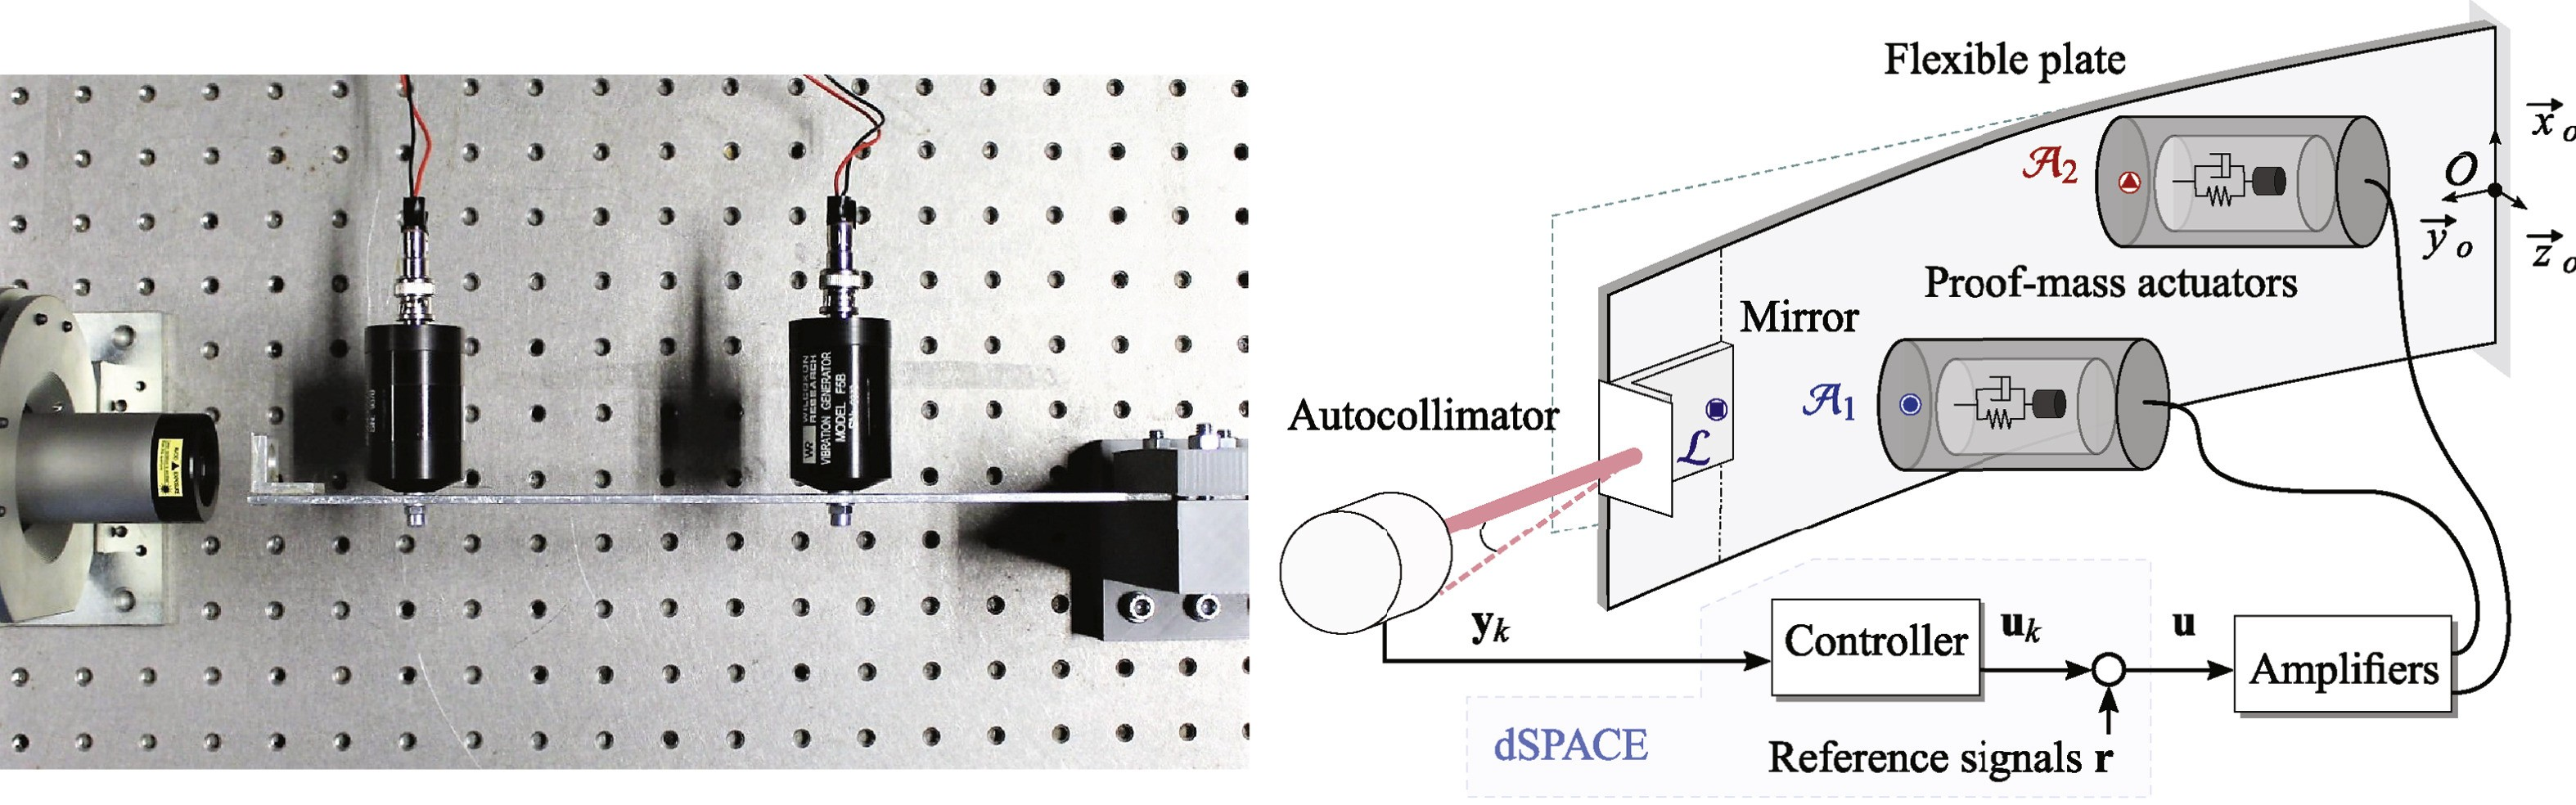
\includegraphics[width=0.95\textwidth]{part_4/validation/KP/setup_sanfe.jpg} 
	\caption{Experimental setup used in \cite{preda2020}. Top down photo of the system (left), schematic diagram of the setup (right).}
	\label{fig:setup_sanfe}
\end{figure}

In this section, the experimental setup presented in \cite{preda2020} is modeled using the pH framework. The setup is composed by a cantilever plate controlled by means of two proof-mass actuators and a mirror used to reflect a laser beam for measuring the end-point deflection (see Fig. \ref{fig:setup_sanfe}).
This system can be constructed modularly considering each component separately. 

\subsubsection{Modular modelling of the system}
In this section, the model for each component is detailed. The final system is obtained by imposing the appropriate transformer interconnections.

\paragraph{Cantilever plate.} The cantilever plate is model as in Sec. \ref{sec:bd_stabKP}. The difference is that now the force at the free boundary are null and that the other components interact with the plate system by means of reaction forces within the domain $\Omega = (0, L_x) \times (0, L_y)$. The forces exerted by the external components can be modelled by a delta distribution. Then the continuous model can be written as the following distributional system

\begin{equation}
\begin{aligned}
\begin{bmatrix}
\rho h & 0 \\ 
\bm{0} & \bm{\mathcal{C}_b} \\
\end{bmatrix}
\diffp{}{t}
\begin{pmatrix}
e_w \\ \bm{E}_\kappa \\
\end{pmatrix} &= 
\begin{bmatrix}
0 & -\div\Div \\ 
\Hess & \bm{0} \\
\end{bmatrix}
\begin{pmatrix}
e_w \\ \bm{E}_\kappa \\
\end{pmatrix} + 
\sum_{i = 1}^{n_{\mathrm{comp}}} 
\begin{bmatrix}
1 & -\partial_y & \partial_x \\
\bm{0} & \bm{0} & \bm{0} \\
\end{bmatrix} \delta(\bm{x} - \bm{x}_{P_i}) \mathbf{u}_{P_i}, \\
\mathbf{y}_{P_i} &= \delta(\bm{x} - \bm{x}_{P_i}) \begin{bmatrix}
1 & \bm{0} \\
-\partial_y & \bm{0} \\
\partial_x & \bm{0} \\
\end{bmatrix}  \begin{pmatrix}
e_w \\ \bm{E}_\kappa \\
\end{pmatrix}, \qquad \forall i \in \{1, n_{\mathrm{comp}}\}
\end{aligned}
\end{equation}
where $n_{\mathrm{comp}}$ is the number of external components, $\bm{x}_{P_i}$ is the attachment point of the $i$-th component, $\mathbf{u}_{P_i} = [F_{P_i}^z \; T_{P_i}^x \; T_{P_i}^y]^\top$ contains the external force along $z$ and the external torques along $x$ and $y$. The torques undergo a derivation, analogously to what happens for the effective shear force at the boundary (cf. Eq. \eqref{eq:effshearforce}). This derivation affects  $\delta(\bm{x} - \bm{x}_{P_i})$, the Dirac delta placed at $\bm{x}_{P_i}$. In the adjoint of the control operator the derivation operator and the Dirac distribution swap their positions
\begin{equation*}
\mathcal{B}_{\Omega, i} =
\begin{bmatrix}
1 & -\partial_y & \partial_x \\
\end{bmatrix} \delta(\bm{x} - \bm{x}_{P_i}), \qquad 
\mathcal{B}_{\Omega, i}^* = \delta(\bm{x} - \bm{x}_{P_i}) \begin{bmatrix}
1 \\
-\partial_y \\
\partial_x \\
\end{bmatrix}.
\end{equation*} 
The model is subjected to the following homogeneous boundary conditions
\begin{align*}
\begin{aligned}
\partial_t e_w|_{\Gamma_D} &= 0, \\
\partial_x e_w|_{\Gamma_D} &= 0, \\
\end{aligned} \qquad 
\begin{aligned}
-\bm{n} \cdot \Div \bm{E}_\kappa - \partial_{\bm{s}} (\bm{E}_\kappa \cddot (\bm{n} \otimes \bm{s}))|_{\Gamma_N}&=0,\\
\bm{E}_\kappa \cddot (\bm{n}\otimes \bm{n})|_{\Gamma_N}&=0, \; \\
\end{aligned} .
\end{align*}
where ${\Gamma_D} = \left\{y = 0 \right\}$, and ${\Gamma_N} = \left\{x = 0 \cup x=L_x \cup y=L_y \right\}$. The flexible plate is then discretized using the Hellan-Herrmann-Johnson elements \ref{eq:HHJ}. The Dirac distribution is approximated by the following boxcar function

\begin{equation}
\delta^{\text{app}}(\bm{x} - \bm{x}_{P_i}) =
\begin{cases}
4 \, h_x h_y, \qquad |x - x_{P_i}| \le h_x \; \text{ and } \; |y - y_{P_i}| \le h_y, \\
0, \qquad \text{elsewhere},
\end{cases}  
\end{equation}
where $h_x, \; h_y$ are the mesh sizes along $x$ and $y$ respectively. In particular 8 elements are taken along the $x$ direction and 60 for the $y$ direction. The following finite-dimensional model is then obtained

\begin{equation}
\begin{aligned}
\mathrm{Diag}
\begin{bmatrix}
\mathbf{M}_{\rho h}\\
\mathbf{M}_{\bm{\mathcal{C}}_b}\\
\mathbf{0}\\
\end{bmatrix}
\begin{pmatrix}
\dot{\mathbf{e}}_{w} \\
\dot{\mathbf{e}}_{\kappa} \\
\dot{\bm{\lambda}}_{\Gamma_D} \\
\end{pmatrix}
&= \begin{bmatrix}
\mathbf{0} & - \mathbf{D}_{\mathrm{HHJ}}^\top & \mathbf{G}_{\Gamma_D}^\top\\
\mathbf{D}_{\mathrm{HHJ}} & \mathbf{0} & \mathbf{0}\\
-\mathbf{G}_{\Gamma_D} & \mathbf{0} & \mathbf{0}\\
\end{bmatrix} 
\begin{pmatrix}
{\mathbf{e}}_{w} \\
{\mathbf{e}}_{\kappa} \\
{\bm{\lambda}}_{\Gamma_D} \\
\end{pmatrix} + \sum_{i = 1}^{n_{\text{comp}}}
\begin{bmatrix}
\mathbf{B}_{\Omega, i} \\
\mathbf{0}\\
\mathbf{0}\\
\end{bmatrix}\mathbf{u}_{P_i}, \\
\mathbf{y}_{P_i}
&= \begin{bmatrix}
\mathbf{B}_{\Omega, i}^\top &  \mathbf{0} &  \mathbf{0} \\
\end{bmatrix}
\begin{pmatrix}
{\mathbf{e}}_{w} \\
{\mathbf{e}}_{\kappa} \\
{\bm{\lambda}}_{\Gamma_D} \\
\end{pmatrix}, \qquad \forall i \in \{1, n_{\text{comp}}\}.
\end{aligned}
\end{equation}
Matrix $\mathbf{D}_{\mathrm{HHJ}}$ represents the discretization of the bilinear form \eqref{eq:bil_HHJ}. Matrix $\mathbf{G}_{\Gamma_D}$ collects the degrees of freedom subjected to the boundary condition. If the degrees of freedom are ordered so that nodes subjected to boundary conditions are place after the non constrained degrees of freedom, this matrix takes the form $\mathbf{G}_{\Gamma_D}= [\mathbf{0} \quad \mathbf{I}]$. Recalling the property of the derivative delta distribution 
$$ \delta'[\phi]  = -\delta[\phi'],$$
where the apostrophe denotes a generic derivative, matrix $\mathbf{B}_{\Omega, i}$ is computed as
\begin{equation}
\mathbf{B}_{\Omega, i}^j = \int_\Omega  \delta^{\text{app}}(\bm{x} - \bm{x}_{P_i}) \begin{bmatrix}
1 & \partial_y & -\partial_x\\
\end{bmatrix} \phi_w^j \d{\Omega}, \qquad \forall j \in \{1,n_w\},
\end{equation}
where $\phi_w^j, \; \forall j \in \{1,n_w\}$ is the test function associated to $e_w$. 

\paragraph{Proof-mass actuator model.}
A proof-mass actuator is mathematically modelled by a hollow cylinder casing of mass $m_{c_i}, \; i \in \{1,2\}$ and inertia with respect to the center of mass $\mathbf{J}_{c_i}=\mathrm{Diag}(J_{c_i}^{xx}, \; J_{c_i}^{yy})$. The casing is connected to a spring-damper-mass system of stiffness $k_i$, damping $c_i$ and internal mass $m_i$. The overall model for this system is the written in co-energies pH form as 

\begin{equation}
\begin{aligned}
\begin{bmatrix}
m_{c_i} & 0 & 0 & 0 & 0\\
0 & {J}_{c_i}^{xx} & 0 & 0 & 0 \\
0 & 0 & {J}_{c_i}^{yy} & 0 & 0 \\
0 & 0 & 0 & m_i & 0 \\
0 & 0 & 0 & 0 & k_i \\
\end{bmatrix}
\begin{pmatrix}
\dot{v}_{c_i} \\
\dot{\omega}_{c_i}^x \\
\dot{\omega}_{c_i}^y \\
\dot{v}_i \\
\dot{\Delta x}_i \\
\end{pmatrix} &= 
\begin{bmatrix}
c_i & 0 & 0 & -c_i & k_i\\
0 & 0 & 0 & 0 & 0 \\
0 & 0 & 0 & 0 & 0 \\
-c_i & 0 & 0 & c_i & -k_i \\
-k_i & 0 & 0 & k_i & 0 \\
\end{bmatrix}
\begin{pmatrix}
{v}_{c_i} \\
{\omega}_{c_i}^x \\
{\omega}_{c_i}^y \\
{v}_i \\
{\Delta x}_i \\
\end{pmatrix}
+ \begin{bmatrix}
1 & 0 & 0 \\
0 & 1 & 0 \\
0 & 0 & 1 \\
0 & 0 & 0 \\
0 & 0 & 0 \\
\end{bmatrix} \mathbf{u}_{A_i}, \\
\mathbf{y}_{A_i} &= \begin{bmatrix}
1 & 0 & 0 & 0 & 0 \\
0 & 1 & 0 & 0 & 0 \\
0 & 0 & 1 & 0 & 0 \\
\end{bmatrix}
\begin{pmatrix}
{v}_{c_i} \\
{\omega}_{c_i}^x \\
{\omega}_{c_i}^y \\
{v}_i \\
{\Delta x}_i \\
\end{pmatrix},
\end{aligned}
\end{equation}
where $v_{c_i}$ is the velocity of the casing at its center of mass, $\omega_{c_i}^x, \; _{c_i}^y$ are the angular velocities of the casing, $v_i$ is the velocity of the internal mass and $\Delta x_i$ is the elongation of the spring. $\bm{u}_{A_i} = [F_{A_i}^z, \;  T_{A_i}^x, \;  T_{A_i}^y]^\top$ are the external forces and torques acting on the casing.

\paragraph{Mirror model.} The mirror is a simple L-shaped rigid body with mass $m_m$, $s_m^x$ static moment and inertia $\mathbf{J}_m = \mathrm{Diag}({J}_{m}^{xx}, {J}_{m}^{yy})$

\begin{equation}
\begin{aligned}
\begin{bmatrix}
m_{m} & s_m^x & 0\\
s_m^x & {J}_{m}^{xx} & 0 \\
0 & 0 & {J}_{m}^{yy} \\
\end{bmatrix}
\begin{pmatrix}
\dot{v}_{m} \\
\dot{\omega}_{m}^x \\
\dot{\omega}_{m}^y \\
\end{pmatrix} &= 
\begin{bmatrix}
1 & 0 & 0 \\
0 & 1 & 0 \\
0 & 0 & 1 \\
\end{bmatrix}\mathbf{u}_M, \\
\mathbf{y}_M &= \begin{bmatrix}
1 & 0 & 0 \\
0 & 1 & 0 \\
0 & 0 & 1 \\
\end{bmatrix}
\begin{pmatrix}
{v}_{m} \\
{\omega}_{m}^x \\
{\omega}_{m}^y \\
\end{pmatrix},
\end{aligned}
\end{equation}

where $v_{m}$ is the velocity of the mirror at its center of mass and $\omega_{c_i}^x, \; _{c_i}^y$ its angular velocities. $\mathbf{u}_M = [F_{M}^z, \;  T_{M}^x, \;  T_{M}^y]^\top$ are the external forces and torques acting on the mirror.

\paragraph{Assembly of the model.} The overall model is obtained interconnecting each components to the others by means of transformer interconnections
\begin{align*}
\begin{aligned}
\mathbf{u}_{P_1} &= - \mathbf{u}_{A_1}, \\
\mathbf{u}_{P_2} &= - \mathbf{u}_{A_2}, \\
\mathbf{u}_{P_3} &= - \mathbf{u}_{M},
\end{aligned}\qquad \qquad
\begin{aligned}
\mathbf{y}_{P_1} &= \mathbf{y}_{A_1}, \\
\mathbf{y}_{P_2} &= \mathbf{y}_{A_2}, \\
\mathbf{y}_{P_3} &= \mathbf{y}_{M}, \\
\end{aligned}\qquad \qquad
\begin{aligned}
\text{First actuator}, \\
\text{Second actuator}, \\
\text{Mirror}. \\
\end{aligned}
\end{align*}



\subsubsection{Numerical results}
The objective is the computation of the natural frequencies to assess the final model in comparison with \cite{preda2020}. For this reason, the damping of the proof-mass actuators is neglected. Once all the components have been assembled together, the overall system takes the form
\begin{equation*}
\mathbf{E} \dot{ \mathbf{x} } = \mathbf{J}\mathbf{x}.
\end{equation*}
where $\mathbf{E} = \mathrm{Diag}(\mathbf{M}, \mathbf{0})$. The parameters of each subsystem, retrieved from \cite{sanfedino2019phd}, are reported in Table \ref{tab:parSetupSanfe}. In Fig. \ref{fig:om_setup} the eigenvectors $\psi_w$ associated to $e_w$ and corresponding eigenfrequencies $\omega_i$ are reported. Their values and corresponding eigenvectors match those reported in \cite{preda2020,sanfedino2019phd}.

\begin{table}[tbh]
	\centering
\begin{tabular}{lllr}
	\hline 
Subsystem	& Parameter  & Description & Value \\ 
	\hline 
\multirow{6}{*}{\shortstack{Flexible \\ Plate}}	& $\rho$  & Density & $2692 \; \mathrm{[kg / m^3]}$ \\ 
	& $E$  & Young modulus  &  $69 \; \mathrm{[GPa]}$\\ 
	& $\nu$ & Poisson's ratio  & 0.33 \\ 
	& $L_y$ & Length & $28 \; \mathrm{[cm]}$ \\ 
	& $L_x$ & Width & $4 \; \mathrm{[cm]}$ \\ 
	& $h$ & Thickness & $3 \; \mathrm{[mm]}$ \\ 
	\hline 
\multirow{7}{*}{\shortstack{Proof-mass\\ Actuators}} & $m_i$ & Mass of the moving mass & $23.6 \; \mathrm{[g]}$ \\ 
	& $m_{c_i}$ & Casing mass  & $182.7 \; \mathrm{[g]}$ \\ 
	& $J_{c_i}^{xx} $ & Casing inertia along $x$  & $0.3 \; \mathrm{[g \cdot m^2]}$ \\ 
    & $J_{c_i}^{yy} $ & Casing inertia along $y$  & $0.3 \; \mathrm{[g \cdot m^2]}$ \\ 
	& $k_i$ & Stiffness  & $1026 \; \mathrm{[N/m]}$ \\ 
	& $\bm{x}_{A_1}$ & Location 1st actuator & $[-1 \quad 25 \quad 0]^\top \; \mathrm{[cm]}$ \\ 
	& $\bm{x}_{A_2}$ & Location 2st actuator & $[1 \quad 10.5 \quad 0]^\top \; \mathrm{[cm]}$ \\ 
	\hline 
\multirow{5}{*}{Mirror}	& $m_{m} $ & Mass  & $23.4 \; \mathrm{[g]}$ \\ 
	& $s_{m}^{x} $ & Static moment  & $-0.338 \; \mathrm{[g \cdot m]}$ \\ 
	& $J_{m}^{xx} $ & Mirror inertia along $x$  & $0.008 \; \mathrm{[g \cdot m^2]}$ \\
	& $J_{m}^{yy} $ & Mirror inertia along $y$  & $0.058 \; \mathrm{[g \cdot m^2]}$ \\
	& $\bm{x}_{M}$ & Location mirror & $[0 \quad 28 \quad 0]^\top \; \mathrm{[cm]}$ \\  
	\hline 
\end{tabular} 
\caption{Parameters for each subsystem}
\label{tab:parSetupSanfe}
\end{table}


\begin{figure*}[p]
	\centering
	\subfloat[1st bending mode $\omega_1 = 10.05 \; \mathrm{[Hz]}$]{\includegraphics[width=0.49\linewidth]{part_4/validation/KP/ActuatedPlate1.eps}%
		\label{fig:om1_setup}}
	\hfil
	\subfloat[1st actuator mode $\omega_2 = 32.82 \; \mathrm{[Hz]}$]{\includegraphics[width=0.49\linewidth]{part_4/validation/KP/ActuatedPlate2.eps}%
		\label{fig:om2_setup}} \\
	\subfloat[2nd actuator mode $\omega_3 = 34.84 \; \mathrm{[Hz]}$]{\includegraphics[width=0.49\linewidth]{part_4/validation/KP/ActuatedPlate3.eps}%
	\label{fig:om3_setup}}
	\hfil
	\subfloat[1st torsional mode $\omega_4 = 47.23 \; \mathrm{[Hz]}$]{\includegraphics[width=0.49\linewidth]{part_4/validation/KP/ActuatedPlate4.eps}%
	\label{fig:om4_setup}} \\
	\subfloat[2nd bending mode $\omega_5 = 63.78 \; \mathrm{[Hz]}$]{\includegraphics[width=0.49\linewidth]{part_4/validation/KP/ActuatedPlate5.eps}%
	\label{fig:om5_setup}}
	\hfil
	\subfloat[2nd torsional mode $\omega_6 = 117.80 \; \mathrm{[Hz]}$]{\includegraphics[width=0.49\linewidth]{part_4/validation/KP/ActuatedPlate6.eps}%
	\label{fig:om6_setup}} \\
	\caption{Eigenvectors for the overall system}
	\label{fig:om_setup}
\end{figure*}


\begin{comment}
Omega full lambda 1: 10.05488286658613
Omega full lambda 2: 32.820440166701395
Omega full lambda 3: 34.841016638952
Omega full lambda 4: 47.23797002941684
Omega full lambda 5: 63.78852519981024
Omega full lambda 6: 117.80124510761422
\end{comment}

\section{Conclusion}


In this chapter the proposed formulation for multibody dynamics has been tested. The employment of finite elements leads to large sparse systems to be solved. To limit the computational complexity of these models, model reduction techniques can be incorporated. While for linear pHDAE systems consolidated methodologies exist \cite{egger2018}, for the  non linear differential-algebraic case solutions are not yet available. To avoid the problem of dealing with large-scale systems, spectral methods can be equivalently used to achieve a structure preserving discretization made up of small and dense matrices. 
The time-domain simulations of the resulting systems have been accomplished using ready-to-use solvers. A rigorous numerical analysis represents an important future development. In particular, numerical methods capable of preserving important structural properties in discrete time have been studied for rigid body dynamics \cite{celledoni2018passivity} and generic ODE \cite{kotyczka2019discrete} and DAE \cite{mehrmann2019structurepreserving} pH systems. These methods could be fruitfully employed in the proposed framework. 